\documentclass{article}

\usepackage{amsmath,amsfonts,amsthm,amssymb,amsopn,bm}
% \usepackage{fullpage}
\usepackage[margin=.9in]{geometry}
\usepackage{graphicx}
% \usepackage{fullpage}
% \usepackage[paper=letterpaper,margin=1in,includeheadfoot,footskip=0.25in,headsep=0.25in]{geometry}
\usepackage{url}
\usepackage[usenames,dvipsnames]{color}
% \usepackage[pdfborder={0 0 1},colorlinks=true,citecolor=black,plainpages=false]{hyperref}
\usepackage{fancyhdr}
\usepackage[ruled]{algorithm2e}
% \usepackage{multirow}
\newcommand{\field}[1]{\mathbb{#1}}
\newcommand{\1}{\mathbf{1}}
\newcommand{\E}{\mathbb{E}} % real domain
\newcommand{\e}{\mathbf{e}} % real domain
\newcommand{\V}{\mathbf{V}} % real domain
\newcommand{\X}{\mathbf{X}} % real domain
% \newcommand{\E}{\mathbb{E}} % real domain
\renewcommand{\P}{\mathbb{P}} % real domain
\newcommand{\R}{\field{R}} % real domain
% \newcommand{\C}{\field{C}} % complex domain
\newcommand{\F}{\field{F}} % functional domain

\newcommand{\T}{^{\textrm T}} % transpose


\def\diag{\text{diag}}
\def\vec{\text{vec}}

%% operator in linear algebra, functional analysis
\newcommand{\inner}[2]{#1\cdot #2}
\newcommand{\norm}[1]{\left\|#1\right\|}
\newcommand{\twonorm}[1]{\|#1\|_2^2}
% operator in functios, maps such as M: domain1 --> domain 2
\newcommand{\Map}[1]{\mathcal{#1}}
\renewcommand{\theenumi}{\alph{enumi}} 

\newcommand{\Perp}{\perp \! \! \! \perp}

\newcommand\independent{\protect\mathpalette{\protect\independenT}{\perp}}
\def\independenT#1#2{\mathrel{\rlap{$#1#2$}\mkern2mu{#1#2}}}
\newcommand{\vct}[1]{\boldsymbol{#1}} % vector
\newcommand{\mat}[1]{\boldsymbol{#1}} % matrix
\newcommand{\cst}[1]{\mathsf{#1}} % constant
\newcommand{\ProbOpr}[1]{\mathbb{#1}}
\newcommand{\grade}[1]{\small\textcolor{magenta}{\emph{[#1 points]}} \normalsize}
\date{{}}

\setlength\parindent{0px}

\begin{document}
\title{Homework \#4}
\author{\normalsize{CSE 546: Machine Learning}\\
\normalsize{Michael Ross} }
\maketitle


\section*{Expectation Maximization}
1. \grade{3} \emph{Pandora} is a streaming music company like \emph{Spotify} that was known to buck the collaborative filtering trend\footnote{Methods like matrix completion can leverage massive user-bases rating lots of items, but suffer from the ``cold-start'' problem: you recommend songs based on people's rating history, but to learn who would like a \emph{new} song you need lots of people to listen to that song, but that requires you to suggest it and possibly degrade recommendation performance.} and instead paid an army of employees to create feature vectors for each song by hand. Suppose you work at a Pandora clone and have feature vectors $x_1,\dots,x_n \in \R^d$ for all $n$ songs in your database, and a particular user, for some subset $\mathcal{S} \subset \{1,\dots,n\}$, has listened to song $i \in \mathcal{S}$ exactly $Y_i \in \{1,2,\dots\}$ times. 
You would like to make a playlist for this user so you assume $Y_i$ is Poisson distributed with mean $\E[Y_i | x_i] =: \lambda_i = e^{w^{T} x_i}$ for some weight vector $w \in \R^d$ reflecting the user's preferences. 
That is,
\begin{align*}
p(Y_i=y | x_i, w) = \frac{\lambda_i^y}{y!} e^{-\lambda_i} = \frac{e^{y x_i^T w}}{y!} e^{-e^{w^T x_i}}.
\end{align*}
The maximum likelihood estimator is $\widehat{w} = \arg\max_w \prod_{i \in \mathcal{S}} p(y_i | x_i, w)$.
The idea is that you would then construct a playlist out of the items $i \in \{1,\dots,n\}$ that maximize $x_i^T \widehat{w}$. 
\begin{enumerate}
  \item The estimate $\widehat{w}$ has no closed-form solution. Can the optimization problem be transformed into a \emph{convex} optimization problem? If so, suggest a method of solving for $\widehat{w}$ given $\{(x_i,y_i)\}_{i \in \mathcal{S}}$. (Hint: how do you show a function $f(x)$ is convex?).
  \item You solve for the $\widehat{w}$ for this user and make a playlist for her. 
  Weeks later you look at her listening history and observe that sometimes she listens to a particular set of songs and skips over others, and at some other point she listens to a different set of songs and skips over others. 
  You have the epiphany that users are human beings whose preferences differ with their mood (e.g., music for workouts, studying, being sad, etc.).
  You decide she has $k$ music moods and aim to make $k$ playlists, one for each mood that could be modeled by a different weight vector $w$. The problem is that you don't know which observation $i \in \mathcal{S}$ is assigned to which mood. Describe (in math and words) how you would use the EM algorithm to make these $k$ playlists.  
\end{enumerate}


\section*{Regression with Side Information}

2. \grade{8} In linear regression we have seen how penalizing the $\ell_2$-norm of the weights (Ridge) and $\ell_1$-norm of the weights (Lasso) affect the resulting solutions. 
Using different loss functions and regularizers to obtain different desired behaviors is very popular in machine learning. 
In this problem we will explore some of these ideas by using a general convex optimization solver CVXPY: \url{http://www.cvxpy.org/} to solve the optimization problems we define. 
Using these kinds of general solvers can be slower than a highly tuned custom solver you write yourself (e.g., accelerated gradient descent with a tuned stepsize) but they make it easy to swap out loss functions or regularizers. 
One of the benefits of convex optimization is that no matter which solver or method is used (coordinate descent, SGD, gradient descent, Newton's, etc.) they all converge to the same function value (unlike non-convex optimization in neural networks where the optimization method itself affects the resulting solution).\\

First let's generate some data. 
Let $n=50$ and $f(x) = 10 \sum_{k=1}^4 \1\{x \geq \frac{k}{5}\}$, noting that $f(x)$ is non-decreasing in $x$ (i.e., $f(x) \geq f(z)$ whenever $x \geq z$). 
For $i=1,\dots,n$ let each $x_i=\frac{i-1}{n-1}$ and $y_i = \1\{i \neq 25\} (f(x_i) + \epsilon_i)$ where $\epsilon_i \sim \mathcal{N}(0,1)$.
The case where $i=25$ represents an outlier in the data.\\

In the last homework we solved a problem of the form $\arg\min_\alpha \sum_{i=1}^n \ell(y_i - \sum_{j=1}^n k(x_i, x_j) \alpha_j)$ where $\ell(z) = \ell_{ls}(z) := z^2$ was the least squares loss. 
Least squares is the MLE for Gaussian noise, but is very sensitive to outliers.
A more robust loss is the Huber loss:
\begin{align*}
\ell_{huber}(z) = \begin{cases} z^2 & \text{ if } |z| \leq 1 \\ 2|z| - 1 & \text{otherwise} \end{cases}
\end{align*}  
which acts like least squares close to $0$ but like the absolute value far from $0$.
% We will learn a function $\widehat{f}(x) = \sum_{i=1}^n k_{rbf}(x,x_i) \alpha_i$ where $\alpha \in \R^n$ are the weights on each points $(x_1,\dots,x_n)$.
Moreover, define a matrix $D \in \{-1,0,1\}^{(n-1) \times n}$
\begin{align*}
D_{i,j} = \begin{cases} -1 & \text{ if } i=j \\ 1 & \text{ if } i=j-1 \\ 0 & \text{otherwise} \end{cases}
\end{align*} 
so that for any vector $z \in \R^n$ we have $D z = ( z_2-z_1, z_3-z_2, \dots z_n - z_{n-1})$
In what follows let $k(x,z) = \exp(-\gamma \|x-z\|^2)$ where $\gamma > 0$ is a hyperparameter. 



\begin{enumerate}
  \item As a baseline, let
\[
  \widehat{\alpha} = \arg\min_\alpha \sum_{i=1}^n \ell_{ls}(y_i - \sum_{j=1}^n K_{i,j} \alpha_j) + \lambda \alpha^T K \alpha \ , \quad \quad \widehat{f}(x)=\sum_{i=1}^n \widehat{\alpha}_i k(x_i,x) 
\]
where $K_{i,j} = k(x_i,x_j)$ is a kernel evaluation and $\lambda$ is the regularization constant.
Plot the original data $\{(x_i,y_i)\}_{i=1}^n$, the true $f(x)$, the $\widehat{f}(x)$ found through leave-one-out CV.
(Hint: start with the problem on the homepage of \url{http://www.cvxpy.org/} and modify it as needed.)

\textbf{Answer:}\\
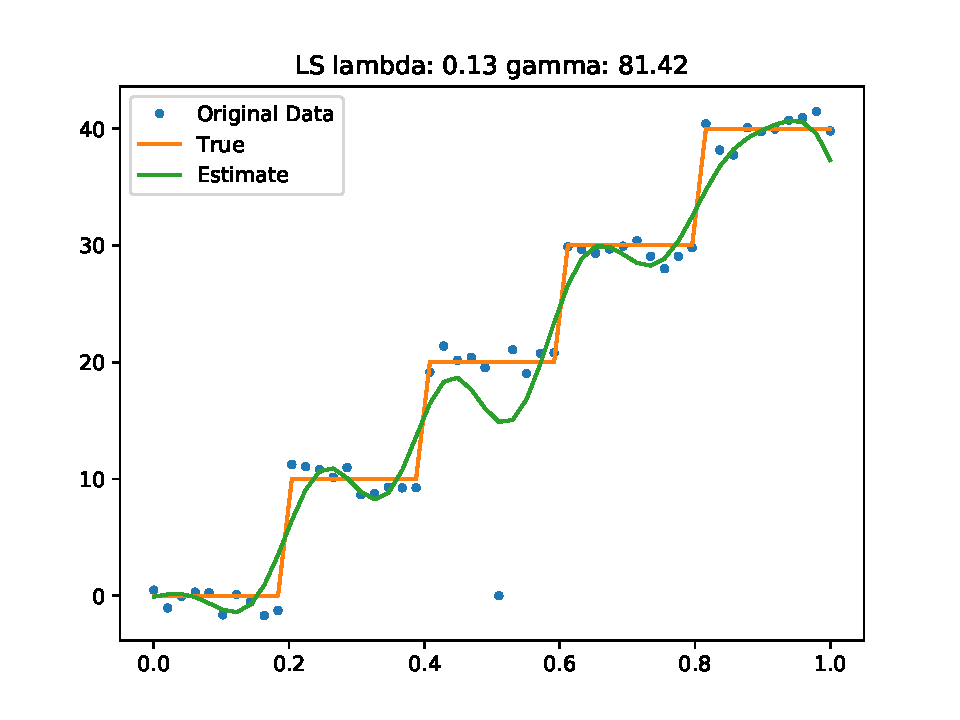
\includegraphics{2_ls.pdf}

\item Now let
\[
  \widehat{\alpha} = \arg\min_\alpha \sum_{i=1}^n \ell_{huber}(y_i - \sum_{j=1}^n K_{i,j} \alpha_j) + \lambda \alpha^T K \alpha \ , \quad \quad \widehat{f}(x)=\sum_{i=1}^n \widehat{\alpha}_i k(x_i,x) 
\]
where $K_{i,j} = k(x_i,x_j)$ is a kernel evaluation and $\lambda$ is the regularization constant.
Plot the original data $\{(x_i,y_i)\}_{i=1}^n$, the true $f(x)$, the $\widehat{f}(x)$ found through leave-one-out CV.
(Hint: \texttt{huber} is a function in \texttt{cvxpy}.)

\textbf{Answer:}\\
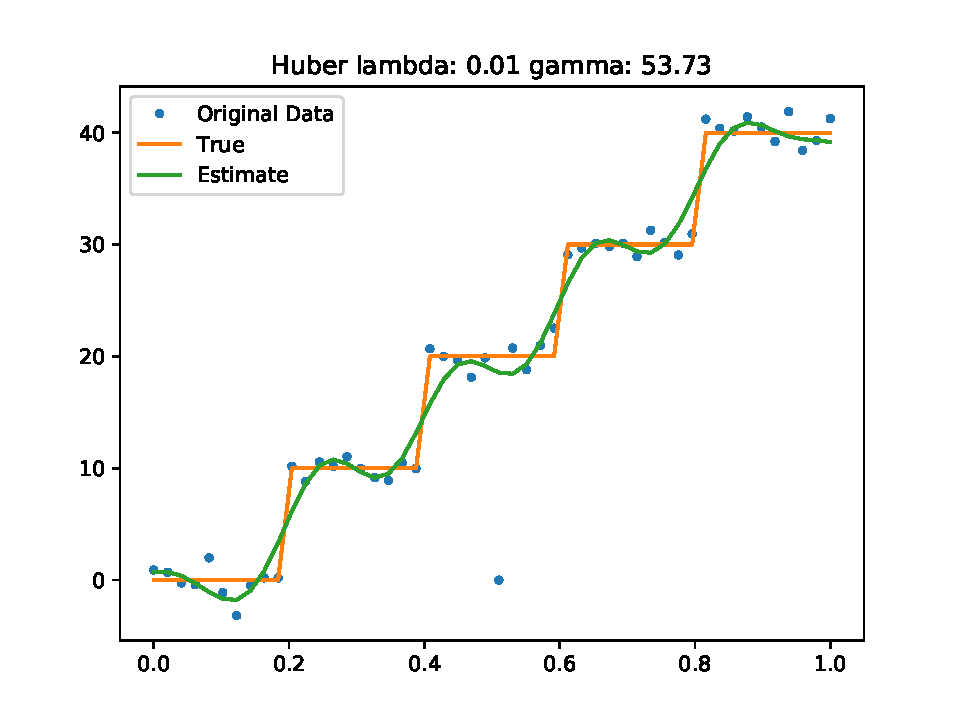
\includegraphics{2_huber.pdf}

  \item The total variation (TV) of a real-valued function $g$ over $\{1,\dots,n\}$ is defined as $\int_{i=1}^{n-1} |g_i - g_{i-1}| = || D g||_1$ and is a common regularizer for de-noising a function (its two-dimensional counterpart is very popular for image de-noising or filling-in missing/damaged parts of photos).   
  Let
\[
  \widehat{\alpha} = \arg\min_\alpha ||K\alpha - y||^2 + \lambda_1 ||D K \alpha||_1  + \lambda_2 \alpha^T K \alpha \ , \quad \quad \widehat{f}(x)=\sum_{i=1}^n \widehat{\alpha}_i k(x_i,x) 
\]
where $K_{i,j} = k(x_i,x_j)$ is a kernel evaluation and $\lambda_1, \lambda_2$ are regularization constants.
For intuition, the penalizer $||D K \alpha||_1$ prefers functions $\widehat{f}$ with sparse jumps in function value while $\alpha^T K \alpha$ perfers functions that are smoothly varying. 
On your own (not necessary to report plots), plot $\widehat{f}$ for a variety values of $\gamma, \lambda_1, \lambda_2$ to see how they affect the solution.
Use leave-one-out cross validation to find a good setting of $\gamma, \lambda_1, \lambda_2$. 
Plot the original data $\{(x_i,y_i)\}_{i=1}^n$, the true $f(x)$, the $\widehat{f}(x)$ found through leave-one-out CV.

\textbf{Answer:}\\
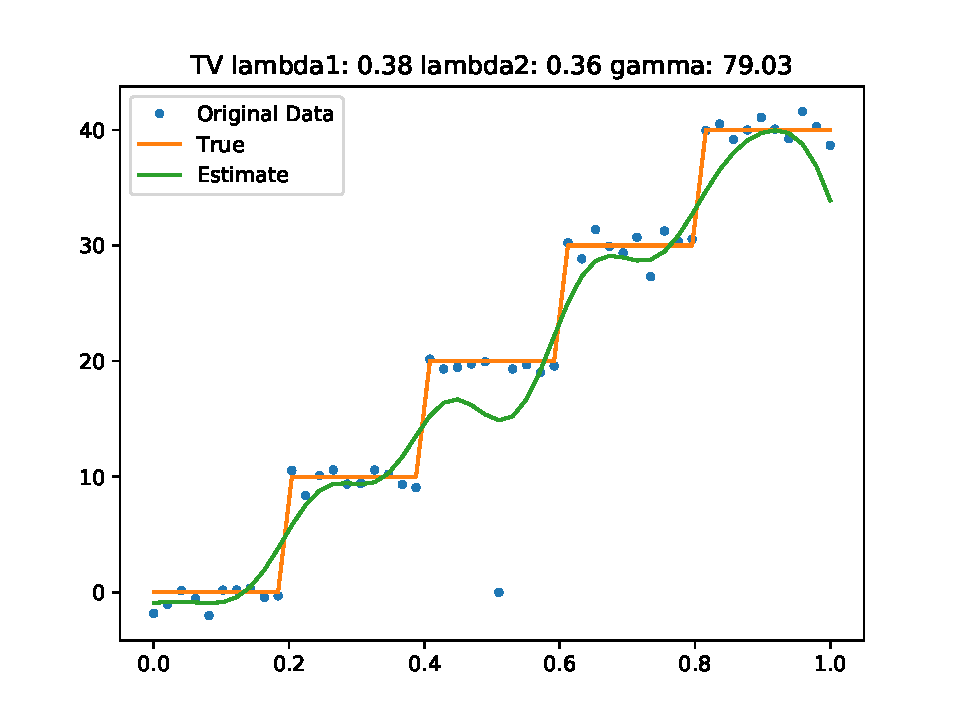
\includegraphics{2_tv.pdf}

\item We say a function $g$ over $\{1,\dots,n\}$ is non-decreasing if $g_i - g_{i-1} \geq 0$ for all $i$, or $D g \geq 0$ where the inequality applies elementwise.
Perhaps due to domain knowledge, we know that the original unnoisy function we are trying to estimate is non-decreasing. 
Let
\begin{align*}
  \widehat{\alpha} &= \arg\min_\alpha ||K\alpha - y||^2  + \lambda \alpha^T K \alpha \ , \quad \quad \widehat{f}(x)=\sum_{i=1}^n \widehat{\alpha}_i k(x_i,x) \\
  & \quad \text{subject to} \quad D K \alpha \geq 0
\end{align*}
where $K_{i,j} = k(x_i,x_j)$ is a kernel evaluation and $\lambda$ is a regularization constant.
The above is known as a quadratic program because it can be written as $\arg\min_x \frac{1}{2} x^T Q x + p^T x +c$ subject to $Ax \leq b$.
On your own (not necessary to report plots), plot $\widehat{f}$ for a variety values of $\gamma, \lambda$ to see how they affect the solution.
Use leave-one-out cross validation to find a good setting of $\gamma, \lambda$. 
Plot the original data $\{(x_i,y_i)\}_{i=1}^n$, the true $f(x)$, the $\widehat{f}(x)$ found through leave-one-out CV.
Note that the defined constraint only forces $\widehat{f}$ to be monotonic on the training data, not over all $x \in [0,1]$, but it is instructive to think about how one might achieve this.

\textbf{Answer:}\\
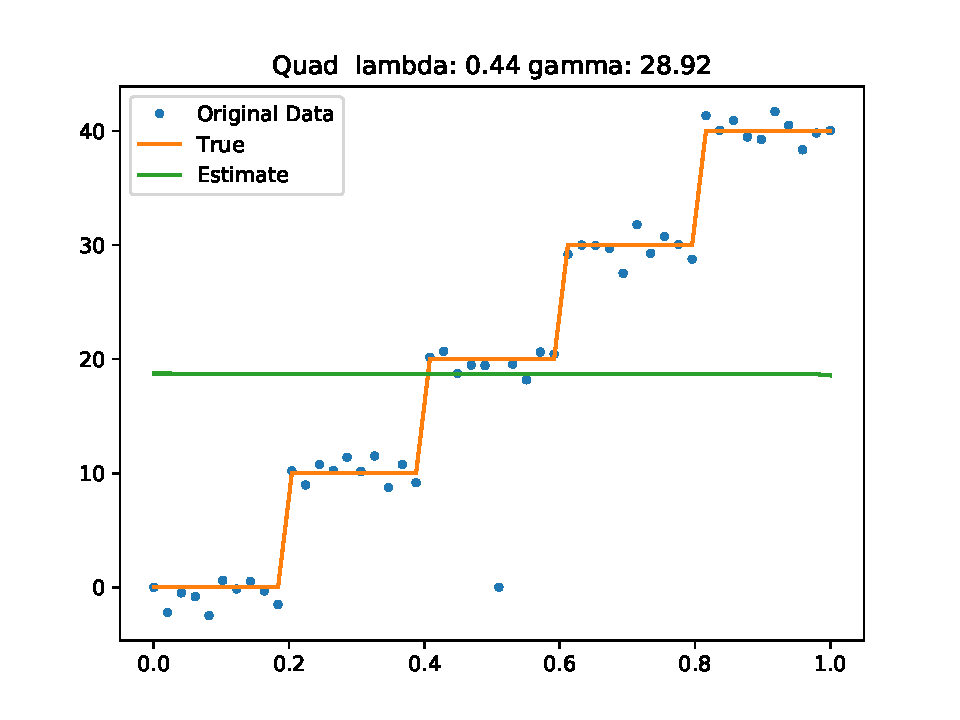
\includegraphics{2_quad.pdf}


\end{enumerate}


\section*{Deep learning architectures}

3. \grade{14} In this problem we will explore different deep learning architectures for a classification task. 
Go to \url{http://pytorch.org/tutorials/beginner/deep_learning_60min_blitz.html} and complete the following tutorials\\[-18pt]
\begin{itemize}
  \item \emph{What is PyTorch?}\\[-18pt]
  \item \emph{Autograd: automatic differentiation}\\[-18pt]
  \item \emph{Neural Networks}\\[-18pt]
  \item \emph{Training a classifier}\\[-18pt]
\end{itemize}
The final tutorial will leave you with a network for classifying the CIFAR-10 dataset, which is where this problem starts. 
Just following these tutorials could take a number of hours but they are excellent, so start early. 
After completing them, you should be familiar with tensors, two-dimensional convolutions (\texttt{nn.Conv2d}) and fully connected layers (\texttt{nn.Linear}), ReLu non-linearities (\texttt{F.relu}), pooling (\texttt{nn.MaxPool2d}), and tensor reshaping (\texttt{view}); if there is any doubt of their inputs/outputs or whether the layers include an offset or not, consult the API \url{http://pytorch.org/docs/master/}. \\

A few preliminaries:
\begin{itemize}
  \item Using a GPU may considerably speed up computations but it is not necessary for these small networks (one can get away with using their laptop).
  \item Conceptually, each network maps an image $x^{in} \in \R^{32 \times 32 \times 3}$ (3 channels for RGB) to an output layer $x^{out} \in \R^{10}$ where the image's class label is predicted as $\arg\max_{i=0,1,\dots,9} x_{i}^{out}$. An error occurs if the predicted label differs from its true label. 
  \item In this problem, the network is trained via cross-entropy loss, the same loss we used for multi-class logistic regression. Specifically, for an input image and label pair $(x^{input}, c)$ where $c \in \{0,1,\dots,9\}$, if the network's output layer is $x^{out} \in \R^{10}$, the loss is $-\log( \frac{\exp(x_c^{out})}{\sum_{c'=0}^9 x_{c'}^{out}})$.
  \item For computational efficiency reasons, this particular network considers \emph{mini-batches} of images per training step meaning the network actually maps $B=4$ images per feed-forward so that $\widetilde{x}^{in} \in \R^{B \times 32 \times 32 \times 3}$  and $\widetilde{x}^{out} \in \R^{B \times 10}$.
  This is ignored in the network descriptions below but it is something to be aware of. 
  \item The cross-entropy loss for a neural network is, in general, non-convex. 
  This means that the optimization method may converge to different \emph{local minima} based on different hyperparameters of the optimization procedure (e.g., stepsize). 
  Usually one can find a good setting for these hyperparameters by just observing the relative progress of training over the first epoch or two (how fast is it decreasing) but you are warned that early progress is not necessarily indicative of the final convergence value (you may converge quickly to a poor local minima whereas a different step size could have poor early performance but converge to a better final value). 
  \item The training method used in this example uses a form of stochastic gradient descent (SGD) that uses a technique called \emph{momentum} which incorporates scaled versions of previous gradients into the current descent direction\footnote{See \url{http://www.cs.toronto.edu/~hinton/absps/momentum.pdf} for the deep learning perspective on this method.}. Practically speaking, momentum is another optimization hyperparameter in addition to the step size. 
  \item We will not be using a validation set for this exercise. Hyperparameters like network architecture and step size should be chosen based on the performance on the test set. This is very bad practice for all the reasons we have discussed over the quarter, but we aim to make this exercise as simple as possible.      
  \item You should modify the training code such that at the end of each epoch (one pass over the training data) compute and print the training and test classification accuracy (you may find the running calculation that the code initially uses useful to calculate the training accuracy).
  \item While one would usually train a network for hundreds of epochs for it to converge, this can be prohibitively time consuming so feel free to train your networks for just a dozen or so epochs. 
\end{itemize}

You will construct a number of different network architectures and compare their performance.
For all, it is highly recommended that you copy and modify the existing (working) network you are left with at the end of the tutorial \emph{Training a classifier}.
For all of the following perform a hyperparameter selection (manually by hand, random search, etc.) using the test set, report the hyperparameters you found, and plot the training and test classification accuracy as a function of iteration (one plot per network).
\textbf{You will receive less credit for very sub-optimal hyperparameter choices that lead to drastically lower error rates than your peers.}
\begin{enumerate}
  \item Fully connected output, 0 hidden layers (logistic regression): we begin with the simplest network possible that has no hidden layers and simply linearly maps the input layer to the output layer. That is, conceptually it could be written as 
  \begin{align*}
  x^{out} = W \vec(x^{in}) +b
  \end{align*} 
  where $x^{out} \in \R^{10}$, $x^{in} \in \R^{32 \times 32 \times 3}$, $W \in \R^{10 \times 3072}$, $b \in \R^{10}$ where $3072 = 32 \cdot 32 \cdot 3$. For a tensor $x \in \R^{a \times b \times c}$, we let $\vec(x) \in \R^{a b c}$ be the reshaped form of the tensor into a vector (in an arbitrary but consistent pattern). 
  \item Fully connected output, 1 fully connected hidden layer: we will have one hidden layer denoted as $x^{hidden} \in \R^{M}$ where $M$ will be a hyperparameter you choose ($M$ could be in the hundreds). The nonlinearity applied to the hidden layer will be the relu ($\mathrm{relu}(x) = \max\{0,x\}$, elementwise). Conceptually, one could write this network as 
  \begin{align*}
  x^{out} = W_2 \mathrm{relu}(W_1 \vec(x^{in}) +b_1) + b_2
  \end{align*}
  where $W_1 \in \R^{M \times 3072}$, $b_1 \in \R^M$, $W_2 \in \R^{10 \times M}$, $b_2 \in \R^{10}$.
  \item Fully connected output, 1 convolutional layer with max-pool: for a convolutional layer $W_1$ with individual filters of size $p \times p \times 3$ and output size $M$ (reasonable choices are $M=100$, $p=5$) we have that $\mathrm{Conv2d}(x^{input}, W_1) \in \R^{(33-p) \times (33-p) \times M}$. 
  Each convolution will have its own offset applied to each of the output pixels of the convolution; we denote this as $\mathrm{Conv2d}(x^{input}, W) + b_1$ where $b_1$ is parameterized in $\R^M$.
  We will then apply a relu (relu doesn't change the tensor shape) and pool. 
  If we use a max-pool of size $N$ (a reasonable choice is $N=14$ to pool to $2 \times 2$ with $p=5$) we have that $\textrm{MaxPool}( \mathrm{relu}( \mathrm{Conv2d}(x^{input}, W_1)+b_1)) \in \R^{\lfloor\frac{33-p}{N}\rfloor \times \lfloor\frac{33-p}{N}\rfloor \times M}$.
  We will then apply a fully connected layer to the output to get a final network given as
  \begin{align*}
  x^{output} = W_2 \vec(\textrm{MaxPool}( \mathrm{relu}( \mathrm{Conv2d}(x^{input}, W_1)+b_1))) + b_2
  \end{align*}
  where $W_2 \in \R^{10 \times M (\lfloor\frac{33-p}{N}\rfloor)^2}$, $b_2 \in \R^{10}$.
  The parameters $M,p,N$ (in addition to the step size and momentum) are all hyperparameters.
  \item (Extra credit: \grade{3}) Returning to the original network you were left with at the end of the tutorial \emph{Training a classifier}, tune the different hyperparameters (number of convolutional filters, filter sizes, dimensionality of the fully connected layers, stepsize, etc.) and train for many epochs to achieve a \emph{test accuracy} of at least 87\%. 
\end{enumerate}
The number of hyperparameters to tune in the last exercise combined with the slow training times hopefully gave you a taste of how difficult it is to construct good performing networks. 
It should be emphasized the networks we constructed are \textbf{tiny}; typical networks have dozens of layers, each with hyperparameters to tune. 
Additional hyperparameters you are welcome to play with if you are so interested: replacing relu $\max\{0,x\}$ with a sigmoid $1/(1+e^{-x})$, max-pool with average-pool, and experimenting with batch-normalization or dropout.


\end{document}
